% Einf�hrungskapitel
%

\chapter{Introduction}

In 2014, the Neurorobotics team of the Blue Brain Project (BBP \cite{BBP}), project of the Ecole Federale Polytechnique Federale de Lausanne (EPFL), successfully produced a point-neuron model
of a mouse brain from data provided by the Allen Institute for Brain Science \cite{AllenInstitute}.
Using the Neural Simulation Tool NEST \ref{NEST}, the BBP Neurorobotics team was able to simulate a
scaled-down model of the mouse brain on a laptop computer, paving the way towards
making a mouse brain interact with an environment. A full-scale implementation of
the mouse brain model is possible, but requires a large scale of resources with low latency requirements that only modern supercomputers can provide today.
The current functionality of NEST generates large neuronal networks on a supercomputer based on only on random distributions, not yet from experimental data contained in brain atlases.
Topic of the thesis is to develop the means to fully model a mouse brain from experimental data using NEST software on available supercomputing architectures.
\newpage

\section{Brain simulation}
\section{Anatomy of the brain}
 
 The human brain is the main part of the central nervous system
 which consists of the spinal cord, sensory organs
 and all of the nerves that connect these organs with the rest of the body.
 These organs are responsible for the control of the body and communication between its parts.
 The nervous system is the most complex system of our body with respect to functionality.
 It contains billions of nerve and glia cells. 
 The nerve cells are connected via synapses to a complex network.
 Electrical pulses from neuron to neuron transmit information through this network.
 Glia cells help maintain the right concentration of chemical substances in the
 extracellular space around neurons and provide supporting structures for the
 growth of neurons and for their spatial arrangement.
  \subsection{Macroscopic structure}
  \label{sec:Macroscopicstructure}
  The anatomy of the brain as depicted in Figure \ref{Aufbau1}, shows that its parts vary in cell density and functionality.
 Figure \ref{Aufbau1} shows a cross-section of the human brain. The outer layer is called gray matter, due to the color caused by the high density of nerve cells.
 For the most port the white matter, which is underneath the gray matter,
 consists mainly of connection fibers of the nerve cells.
 The thalamus is located in the middle of the brain and functions as a relay station between the sensory system and the cortical systems for cognition and motor control.
  \begin{figure}[!htbp]
  %\subfigure[A cross-section of the human brain shows different densities of nerve cells \cite{CN}.]{
  %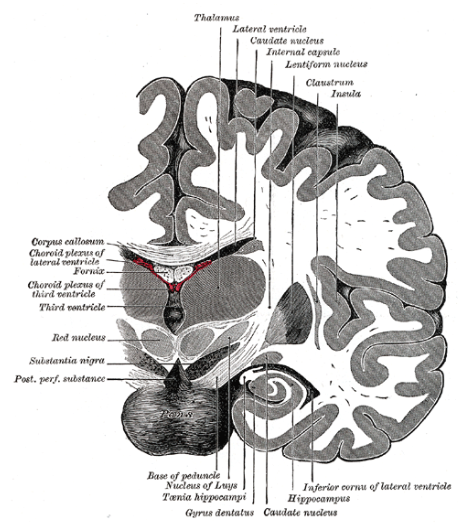
\includegraphics[scale=0.3]{pictures/Aufbau1.png}
  %\label{Aufbau1}
  %}
  \hfill
  \subfigure[A general map of the human brain assigns parts of the gray matter to fuctionalities \cite{CN}.]{
  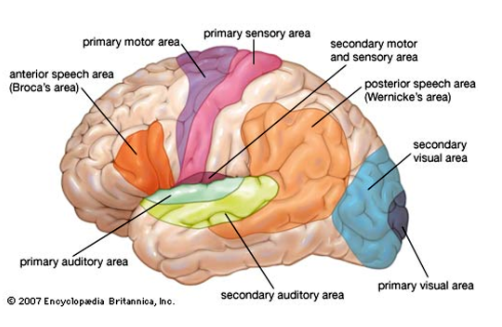
\includegraphics[scale=0.5]{pictures/Aufbau2.png}
  \label{Aufbau2}
  }
  \hfill
  \subfigure[The vertical structure of the gray matter shows six layers \cite{CN}.]{
  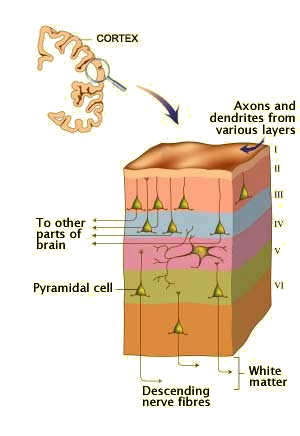
\includegraphics[scale=0.5]{pictures/mikro_aufbau.png}
  \label{mikroaufbau}
  }
  \caption{Macroscopic structure of the human brain.}
  \end{figure}
  Because of the high density of nerve cells the gray matter is the main part of information processing of the brain.
  
  Some parts of the brain can still be assigned roughly to functionality as shown in Figure \ref{Aufbau2}.
  However, the number of nerve cells (neurons), the number of connections (synapses) and the structure differs from person to person.
  The connections of each neuron are dynamic and change over time. \\
  Having a look at the vertical structure of the cortex,
  the gray matter can be partitioned in six layers as shown in figure \ref{mikroaufbau}.
  The cells in each layer have similarities like: cell type, connections to other layers and connections to the thalamus and other parts.
  %-forebrain(anterior part of the brain)
  %-neocortex(surface of the mammalian brain, gray)
 
 
  \newpage
  \subsection{Microscopic structure}
  The nerve cells are tiny structures which are connected to each other.
  In order to understand the brain, a deeper look at the nerve cells is however necessary.
  There are different cell types in a brain. They vary in structure and size.
  Pyramidal, spiny stellate and smooth stellate cells occur most often.
  Each layer has types which occur more frequently.
  
  Figure \ref{Corticalneurons} depicts a typical neuron.
  It contains the soma (the cell body) dendrites and axons.
  Electrical pulses are transported from the dendrites to the soma.
  In case of a spike an electrical impulse is forwarded through the axon.
  These axons are connected via synapses to further dendrites.
  Electrical impulses are transmitted via either chemical reactors (chemical synapses)
  or electrical contacts (gap junctions) between the axons and dendrites.
  \begin{figure}[!htbp]
    \centering
    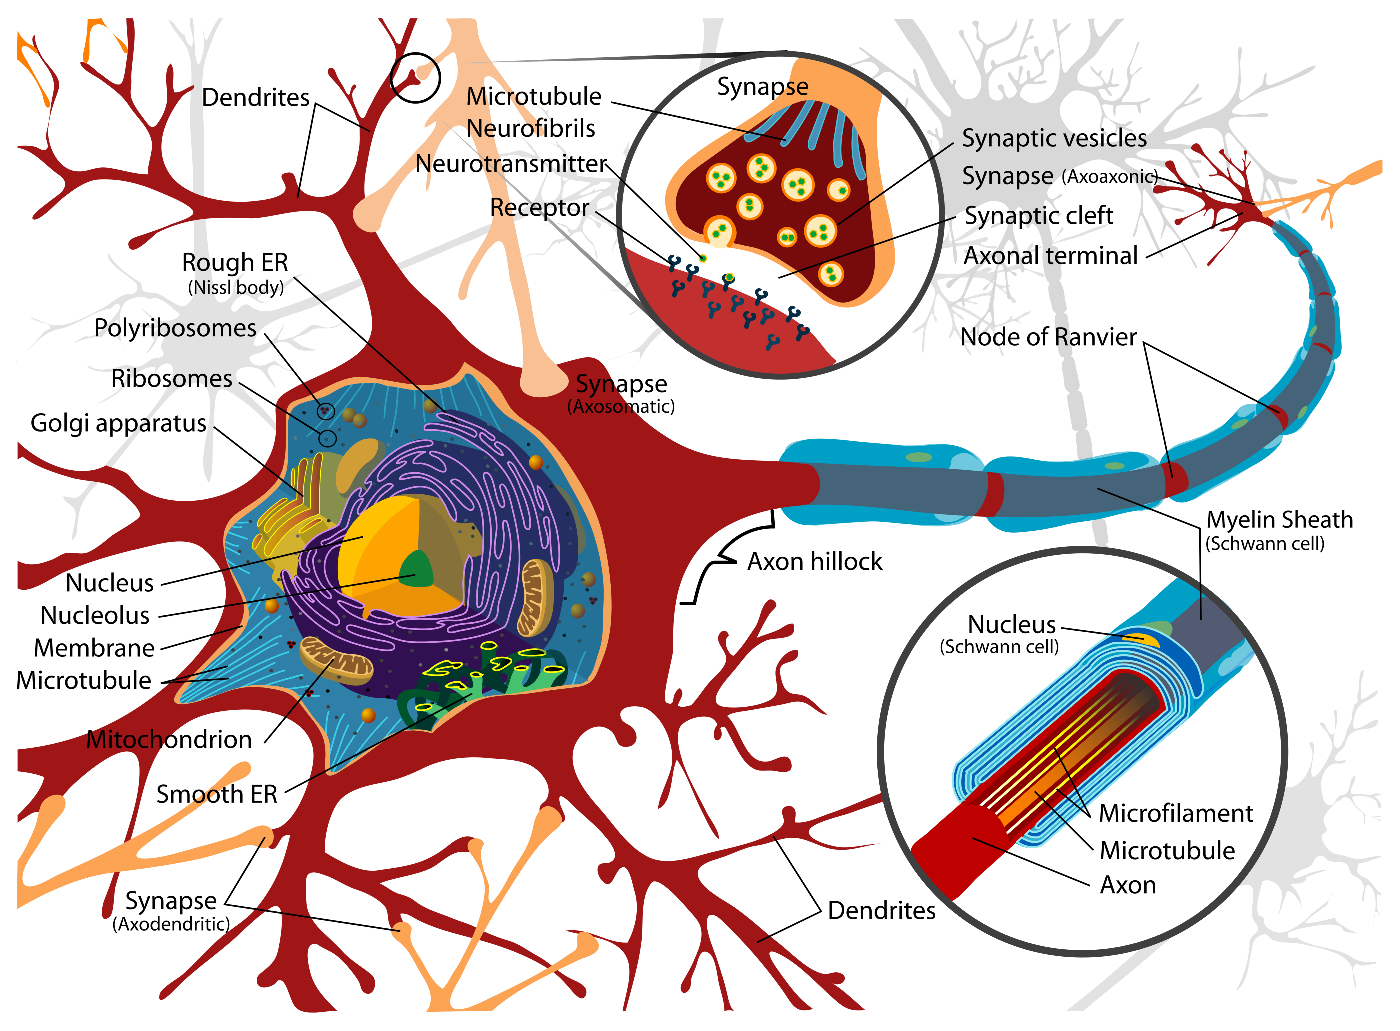
\includegraphics[scale=0.65]{pictures/Complete_neuron_cell_diagram_en.eps}
    \caption{Microscopic structure of a neuron. \cite{neuronpic}}
    \label{Corticalneurons}
  \end{figure}
  There are excitatory and inhibitory neurons.
  The excitatory neurons excite the following neurons, 
  in contrast the inhibitory neurons inhibit the following neurons.
  Via electrical currents the connected neurons influence the membrane potential of each neuron.
  , which can be measured.
  For example, Figure \ref{membrane_potential} shows the membrane potential plotted over time.
  Chemical processes inside the neuron generate a spike if the membrane potential reaches a specific electrical level called the threshold.  
  As shown in Figure \ref{membrane_potential} spikes are peaks in the membrane potential.  
  
  %-cortical neurons
  %-different cells: pyramidal, spiny stellate, smooth stellate
  %-cortical layers
  %-synapses
  
  %-10e12 neurons in the human brain
  \begin{figure}[!htbp]
  \subfigure[Membrane potential of a neuron over the time.
  The peaks are called spikes.
  There are four spikes in the time span shown.
  The firing threshold of the cell is at about 58 mV \cite{CN}.]{
  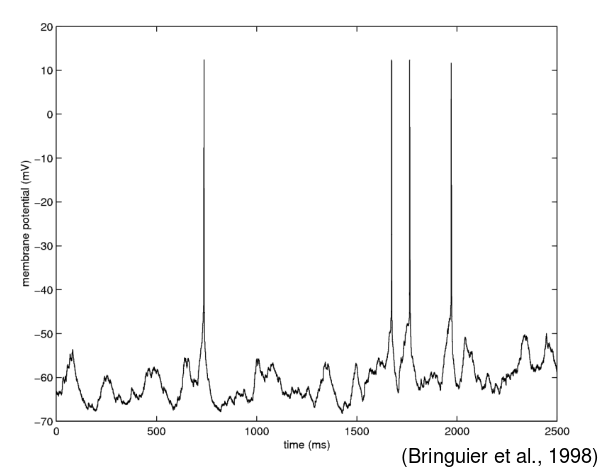
\includegraphics[scale=0.36]{pictures/membrane_potential.png}
  \label{membrane_potential}
  }
  \hfill
  \subfigure[The dot plot shows spikes of each neuron over time. On the y-axis there are the neurons number.
  The histogram in the lower panel sums up all spikes for each time bin. \cite{CN}]{
  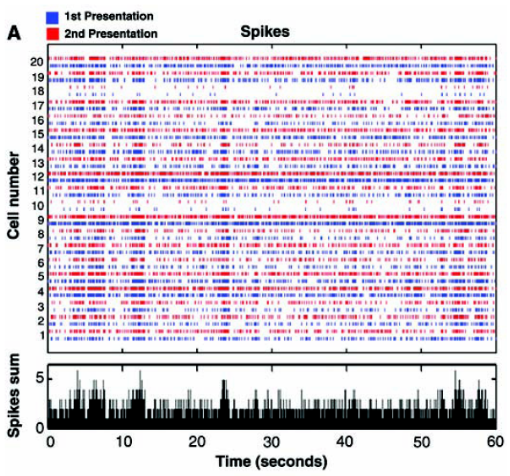
\includegraphics[scale=0.36]{pictures/spike_plot.png}
  \label{spikeplot}
  }
  \end{figure}
  
  In order to analyse the membrane potential more objectively it is reduced to timings of the spikes.
  For multiple neuron the spike timings in a dot plot can be visualized as in Figure \ref{spikeplot}.
  One can get an overview of the activity in a whole neuronal network if the spike sums are
  plotted (summed up spikes for each time bin) in a histogram (bottom row of figure \ref{spikeplot}).

	\begin{itemize}
      \item Short overview over simulators: NEST, NEURON, STEPS
      \item Possibilities/limits of simulations
   \end{itemize}
   
\section{Virtual mouse}
	\begin{itemize}
      \item Available data
      \item Why of interest
   	\end{itemize}   
\newpage
\section{Allen Brain Atlas}
   Allen Institute for Brain Science provides a high-resolution map of neural connections in the mouse brain.
   It contains several injection experiments (see Figure \ref{fig:atlas}). The provided datasets of the experiments 
   contain a 3D image of cell injection and a 3D image of its axonal projection labelled by viral
   tracers.
   
   \begin{figure}[ht!]
   	\begin{center}
        \subfigure[Injection sites - showing all available experiments]{%
            \label{fig:allInjections}
            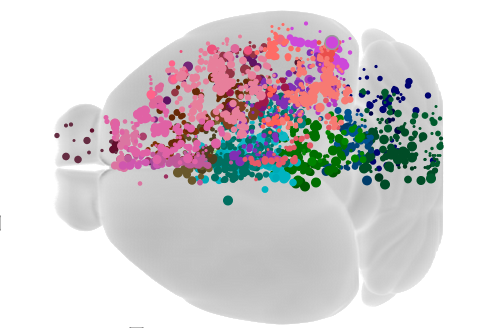
\includegraphics[width=0.4\textwidth]{pictures/connectionBrowser_allinjections.png}
        }
        \hspace{1cm}
        \subfigure[Projection density of one experiment]{%
            \label{fig:oneProjection}
            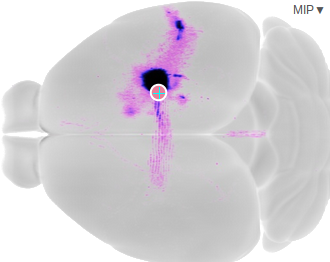
\includegraphics[width=0.32\textwidth]{pictures/connectionBrowser_oneinjections.png}
       }
   	\end{center}
    	\caption{%
         Illustration of the given experiments and the projection image of an example experiment.
   		 It gives an insight into the synaptic structure of the whole brain.
     }%
   \label{fig:atlas}
   \end{figure}
   The images provide connection information between neurons all over the brain.
   The extracted connectivity information is used to build of long range connectivity inside
   the mouse brain model.
   \begin{figure}[ht!]
   	\begin{center}
        \subfigure[Illustration injection]{%
           \label{fig:allInjections}
           
\includegraphics[width=0.15\textwidth]{pictures/cg_illustration_injection.eps}
        }
        \hspace{0.5cm}
        \subfigure[Illustration projection]{%
            \label{fig:oneProjection}
            
\includegraphics[width=0.15\textwidth]{pictures/cg_illustration_projection.eps}
       }
       \hspace{0.5cm}
       \subfigure[Merge experiment]{%
            \label{fig:allInjections}
            
\includegraphics[width=0.15\textwidth]{pictures/cg_illustration_merge.eps}
        }
        \hspace{0.5cm}
        \subfigure[specify source and target neurons]{%
            \label{fig:oneProjection}
            
\includegraphics[width=0.15\textwidth]{pictures/cg_illustration_neurons.eps}
       }
    \end{center}
    	\caption{%
        Assign density of experiments to neurons.
     }%
   \label{fig:atlasvoxel}
   \end{figure}

The 3D images contain discrete voxelized density values.
Most entries are zero. All entries which are above a given threshold are interpreted 
as injected and projected voxels.
Using a piecewise constant interpolation the values are assigned to each neuron.
So for one experiment source and possible target neurons are specified (see Figure \ref{fig:atlasvoxel}).
A set of experiments is used to connect neurons located at the injections
to the neurons at the projections. Because multiple experiments have injected the same regions and therefore
same neurons, for each neuron the experiment is used which has the lowest total injection
density (sum of all injection densities).
The algorithm iterates over all experiments and determines its
total injection. Inside it iterates over all injected voxels.
If there are not connections generated yet for the current voxel or the previous connections
where generated with an experiment having a higher total injection density the connections are regenerated.
For each voxel it iterates over all containing neurons.
For each neuron $10,000$ (source neuron) connections are generated to neurons (target neurons) in the experiment projection area.
	The target neurons are randomly (taking each probability value into account) picked
	out of all possible neurons inside the projection area.
	The delay is determined based on the distance of the source and target neuron.
	Further parameters are determined with a specific direct function and a random variable.
   
   \begin{algorithm}
	\KwData{Injection experiments}
	\KwResult{Long range synapses}
	\For{each experiment}{
		identify the corresponding rAAV
		\For{each injected voxel}{
			\If{rAAV smaller than one used before}{
				\For{each neuron n in voxel}{
					Select all neurons in the projection area; \\
					Assign each of them the normalized intensity value $D_i$ of the voxel they are situated in \\
					Generate a random number P between 0 and 1; \\
					Pick randomly a neuron i; \\
					\If{$P < D_i$}{
						Create an efferent synapse from the selected neuron to neuron $i$; \\
						Assign synaptic parameters; \\
					}
					Repeat from step 4) until Nsy=10000 efferent synapses are assigned	;
				}
			}
		}
	}
\label{alg2}
\caption{Generate long range connectivity}
\end{algorithm}
   
   \newpage
\section{Blue Brain Project recipe}

The Blue Brain Project was able to reconstruct a microcircuit of part of somatosensory cortex of a juvenile rat \cite{markram2015reconstruction}.
They presented a complementary algorithmic approach that reconstructs neuronal microcircuitry
across all layers using available sparse data and that leverages biological principles and
interdependencies between datasets to predict missing biological data.
The algorithm with the available data form a recipe which is applied to the mouse
brain model to estimate the short range connectivity inside the mouse neocortex.
\begin{figure}[ht!]
\centering
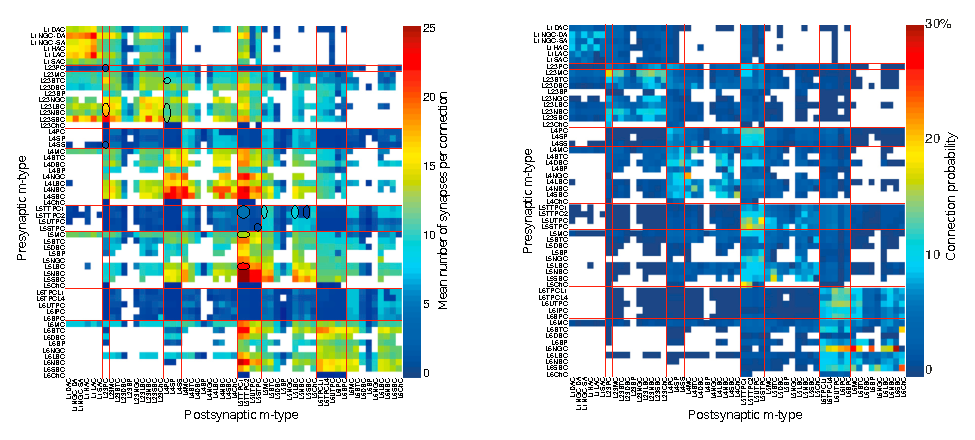
\includegraphics[scale=0.9]{pictures/BBPconnectionPropasMatrix.eps}
\caption{(Left) Synapses per connection. A matrix of the average synapses per connection for multi-synapse connections formed between the 55 m-types.
(Right) Connection probabilities. A matrix of average connection probabilities within 100 mm.}
\label{BBPconnectionPropasMatrix}
\end{figure}
The recipe is mainly based on connection probabilities of different neuron types inside the somatosenory cortex.
To a given point neuron cloud with neuron type information the recipe returns synaptic
connection details (e.g matrices in Figure \ref{BBPconnectionPropasMatrix} shows the number of connections and connection probability between two neurons concerning their \emph{m-type}), which are used to extent the long range connectivity from the Allen Brain Atlas by short range connectivity. 
\begin{figure}[ht!]
   	\begin{center}
        \subfigure[contain all neuron information]{%
            \label{fig:shortColumn}
            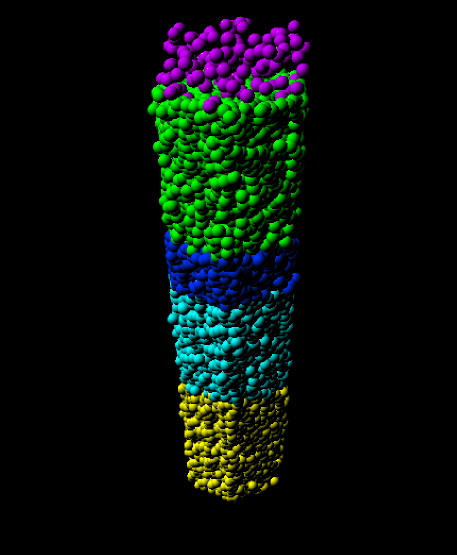
\includegraphics[width=0.22\textwidth]{pictures/g3111.png}
        }
        \hspace{0.5cm}
        \subfigure[contain all synapse information]{%
            \label{fig:shortColumnInCircuit}
            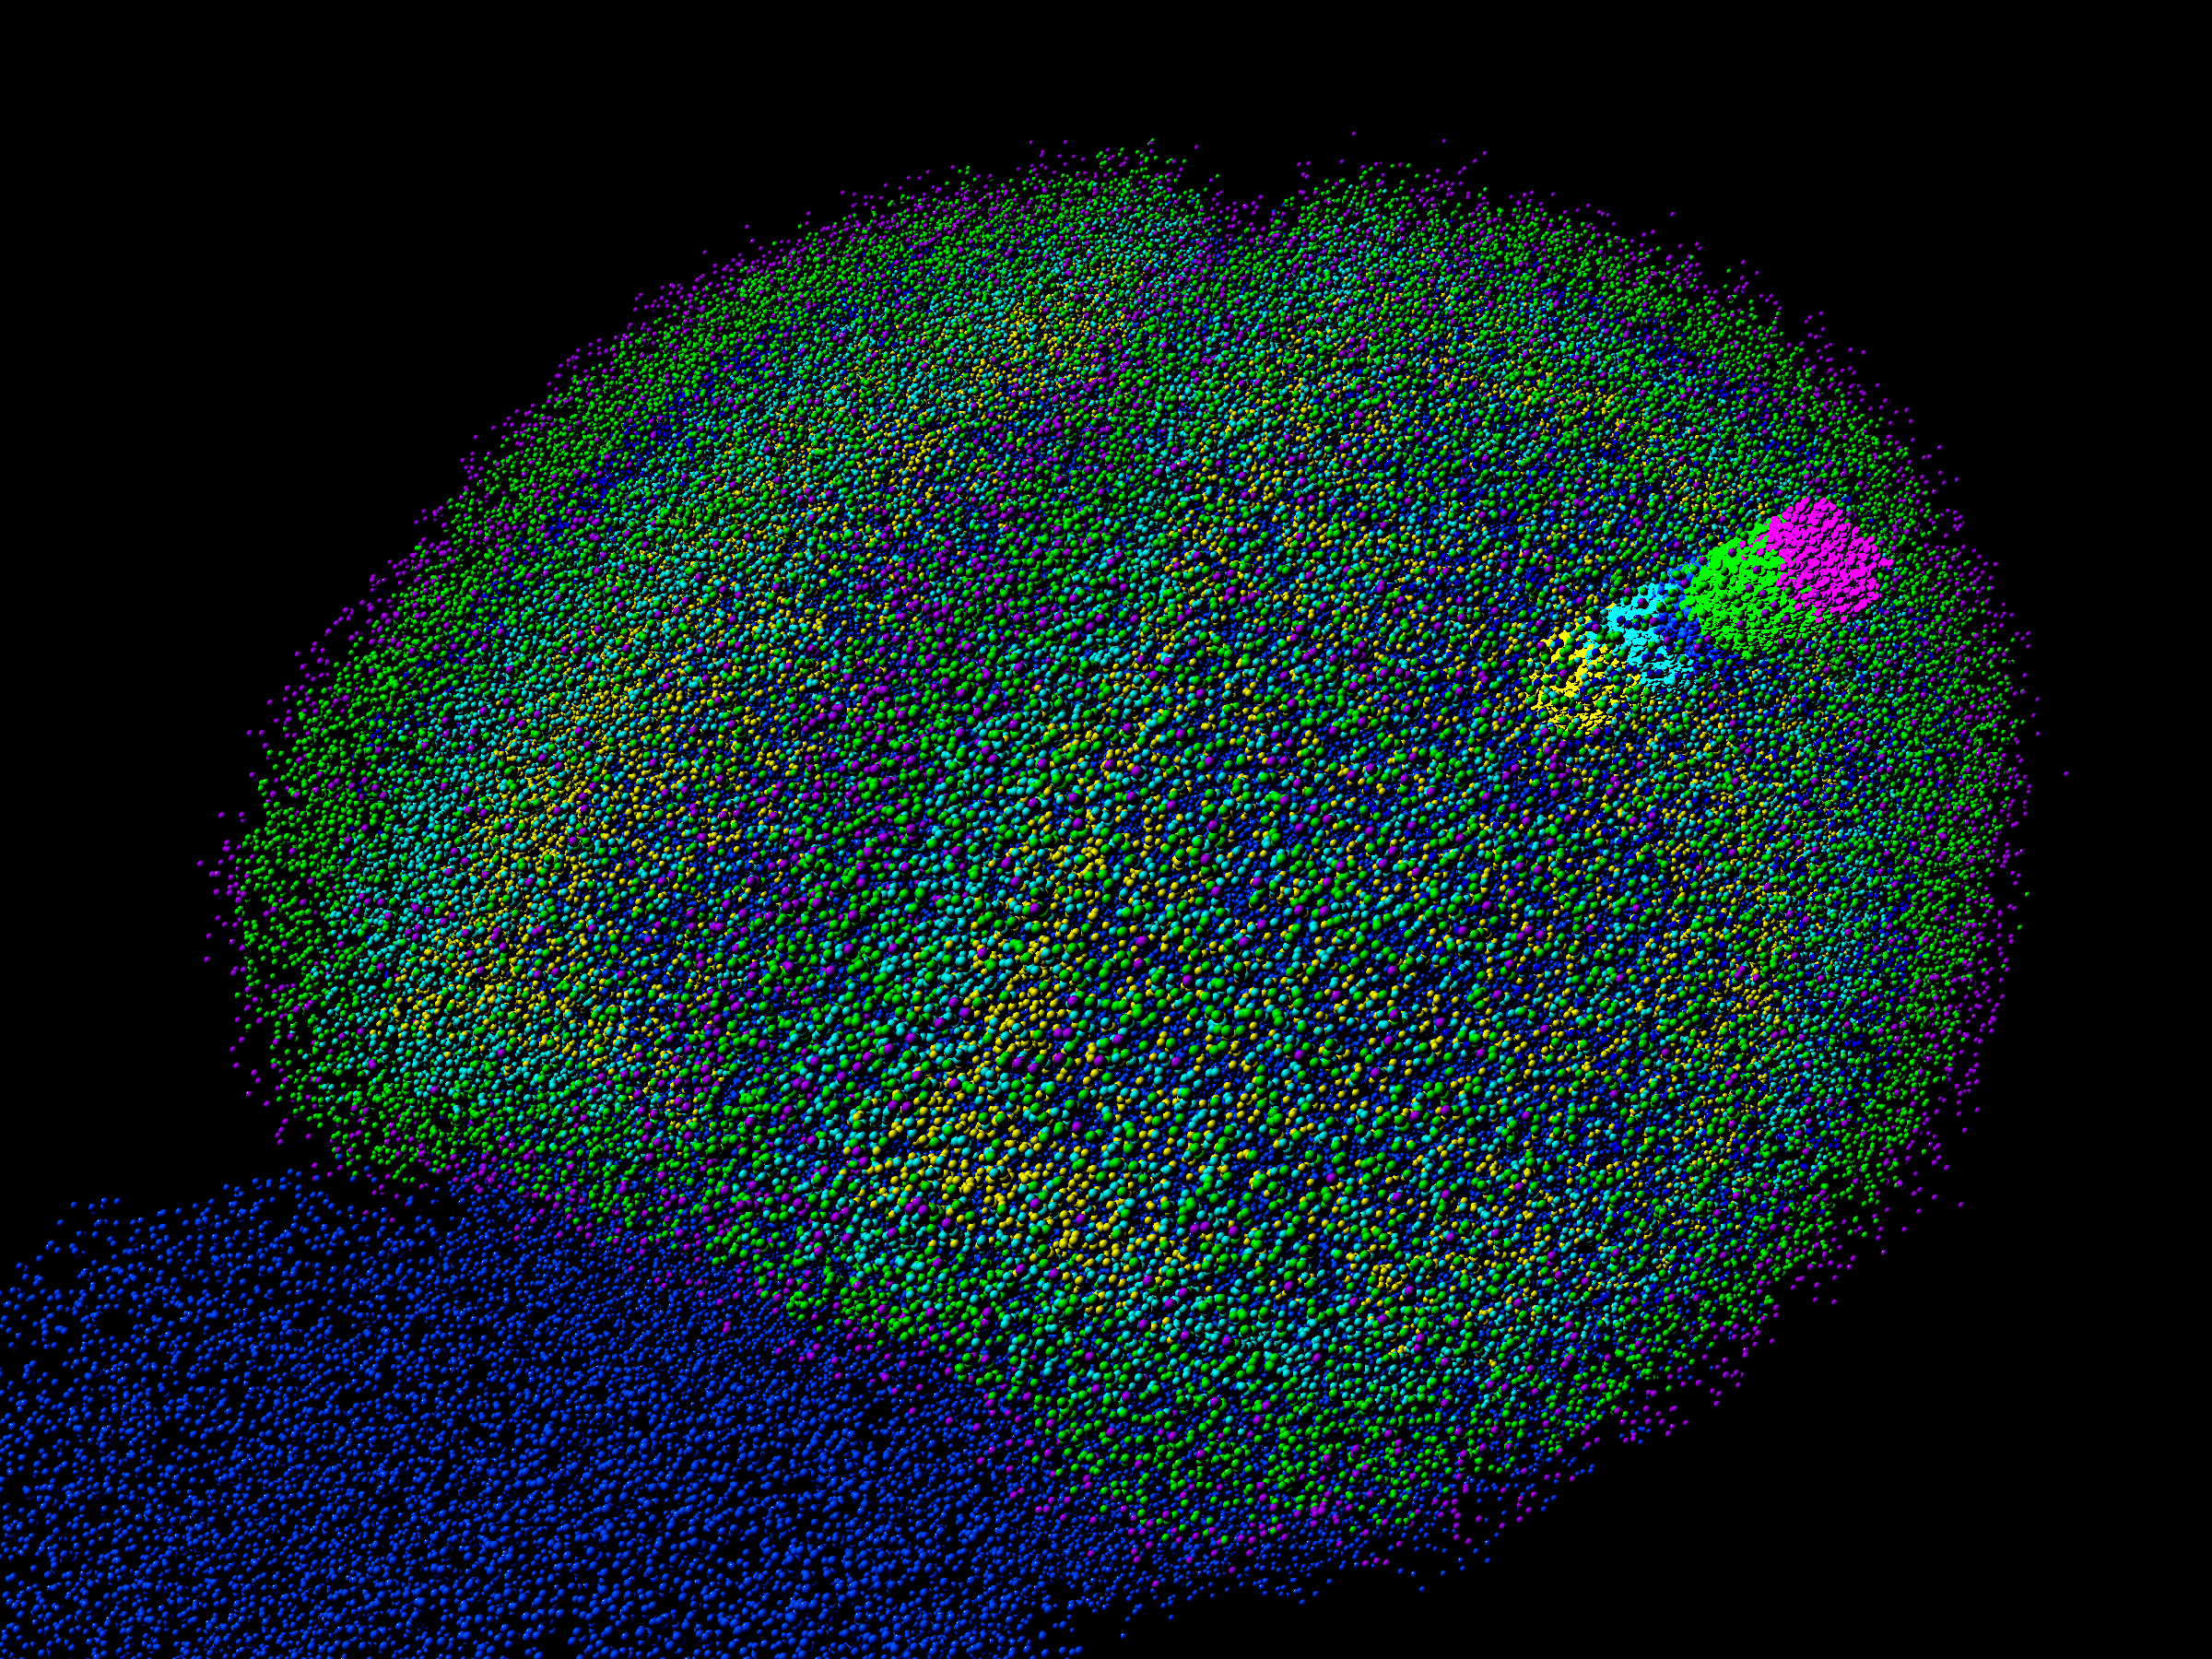
\includegraphics[width=0.34\textwidth]{pictures/column_in_brain_4_edit.png}
       } 
    	   \end{center}
    	\caption{%
        3D visualization of the original Blue Brain Project column (left) and the reconstructed mouse
isocortical column that has a similar neuron density (right). Layers 1, 2/3, 4, 5 and 6 are
shown in different colors.
     }%
   \label{fig:atlas}
   \label{fig:shortColumnInCircuit}
\end{figure}
The given generation script loads needed neuron parameters (layer, m-type,
e-type, coordinates,..) from the HDF5 file\ref{fig:allInjections}.
After that it iterates over all neurons inside the neocortex region
(neurons which are in layer 1 to 6 specified with the parameter layer).
For each neuron (source neuron) all neurons (target neurons) inside its surrounded column
(see geometrical illustration in Figure \ref{fig:shortColumn} and voxelized 2D illustration in
Figure \ref{illcolumn}) are selected.
\begin{figure}[ht!]
\centering

\includegraphics[scale=2.5]{pictures/illustration_shortrange_select.eps}
\caption{Illustration of neurons in column on grid}
\label{illcolumn}
\end{figure}
A random number $P$ is generated and a neuron is picked randomly from the selection.
The neurons acceptance value $D_i$ is determined from the given BBP matrices.
If it is below $P$ a connection between the two neurons is created.
Therefore all synaptic parameters are determined from the BBP matrices.
   \begin{algorithm}[ht!]
	\KwData{BBP matrices}
	\KwResult{Short range synapses}
	\For{each neuron n}{
		Select all neurons in neuron $i$ column area; \\
		Generate a random number P between 0 and 1; \\
		Pick randomly a neuron j from selected area; \\
		Determine $D_i$ based on BBP matrices (neuron i properties, neuron j properties); \\
		\If{$P < D_i$}{
			Create an efferent synapse from neuron $i$ to neuron $j$; \\
			Assign synaptic parameters; \\
		}
	}
\caption{Short range generation algorithm}
\label{alg:BBP}
\end{algorithm}
\newpage
\section{Neural Simulation Tool}
\label{NEST}
Neural Simulation Tool, NEST, is a simulator for spiking neural network models that focuses on the dynamics, size and structure of neural systems rather than on the exact morphology of individual neurons. The development of NEST is coordinated by the NEST Initiative. NEST is used to model networks with simplified morphologies of spiking neurons of any size. For example it is used for
models of information processing e.g. in the visual or auditory cortex of mammals, models of network activity dynamics, e.g. laminar cortical networks or balanced random networks and models of learning and plasticity. A NEST simulation tries to follow the logic of an electrophysiological experiment that takes place inside a computer with the difference, that the neural system to be investigated must be defined by the experimenter. The definition is based on number of neurons with parameters and connections between these neurons. NEST supports the generation based on probabilistic values. The stochastic settings of a neuronal network can be used to create its artificial copy inside of NEST. To manipulate or observe the network dynamics, the experimenter can define devices which represent the various instruments (for measuring and stimulation) found in an experiment. These devices write their data either to memory or to file. 

NEST features the execution on parallel environments (e.g. super computers as JUQUEEN).
Therefore it uses the MPI (Message Passing Interface \cite{MPI}) standard for interprocess communication.
For thread parallelism it supports PThreads\cite{pthread} and OpenMP\cite{openmp}.


\newpage
\subsection{Data structure}
\label{sec:NEST:Datastructure}
NEST keeps the full neuronal network model in memory.
Therefore it distinguishes between nodes and connections.
Nodes and connections represent mostly neurons and synapses, respectively.
Nodes hold model parameters.
However synapses hold besides model parameters the pre-synaptic and post-synaptic neuron information, which each synapse connects.

In multi process environments nodes are distributed on the processes.
For multi threaded environments each thread processes a subset of nodes.
Each process holds a list of meta information of all neurons.
However the model objects are only stored on one process.
Node $i$ is stored on process $p_i$ (\ref{eq:processfromid}) and is processed by thread $t_i$ (\ref{eq:threadfromid}).
\begin{equation}
 	p_i = i \bmod N_{processes}
 	\label{eq:processfromid}
\end{equation}
\begin{equation}
 	t_i = \frac{i}{N_{processes}} \bmod N_{threads}
 	\label{eq:threadfromid}
\end{equation}
$N_{processes}$ and $N_{threads}$ corresponds to the number of processes and number of threads, respectively.
\begin{figure}[ht!]
\centering
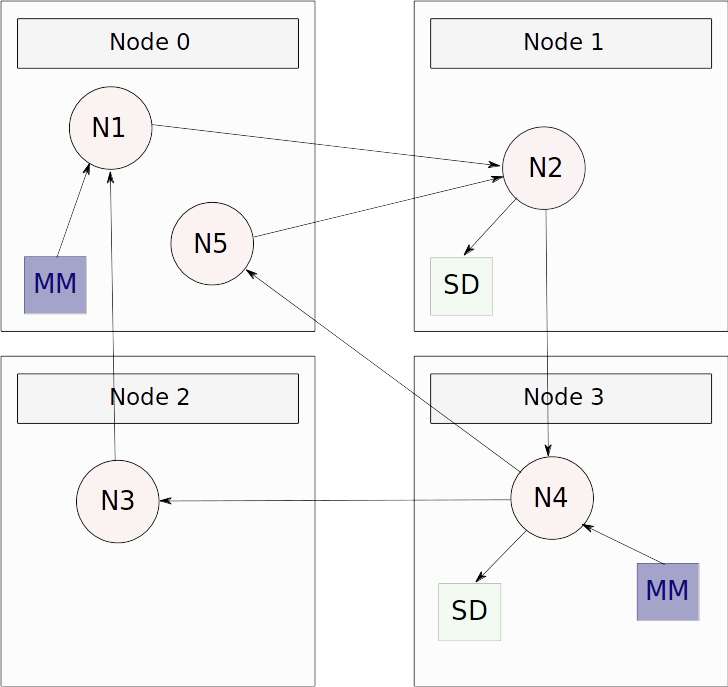
\includegraphics[scale=0.3]{pictures/NeuronsOnNodes.png}
\caption{Illustration how NEST distributes nodes on processes based on their id}
\label{fig:NeuronsOnNodes}
\end{figure}
Figure \ref{fig:NeuronsOnNodes} illustrate the distribution of node model objects on
the different processes.
Synapses are stored on the thread (or process for environments without thread parallelisms) where the post-synaptic node is placed.
Each thread holds a sparse table \ref{fig:NESTsynstorage} containing all
local synapses.
\begin{figure}[ht!]
\centering
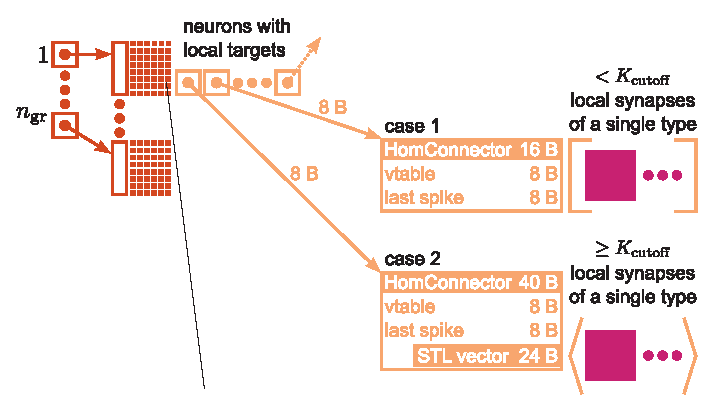
\includegraphics[scale=0.9]{pictures/NEST_syn_storage.eps}
\caption{A sparse table
(dark orange structure and attached light orange boxes with arrows) holds the
thread-local connection objects (pink squares) sorted according to the global
index of the associated pre-synaptic node. The sparse table consists of $n_{gr}$
equally-sized groups, where each group maintains a bit field (tiny squares)
with one bit for each global node index in the group indicating the presence
or absence of local targets. If a particular node has local targets, the sparse
table stores a pointer to an additional inner data structure (light orange)
Auto-adjusting connection infrastructure of NEST.
Case 1: A particular node has less than $K_{cutoff}$
local connections and all are of the same type. A lightweight inner structure
(HomConnector) stores the connection objects in a fixed-size array.
A particular node has at least $K_{cutoff}$
local connections and all are of the same type. A HomConnector stores the
connection objects in a dynamically-sized vector (copied and simplified from \cite{kunkel2014spiking}).
}
\label{fig:NESTsynstorage}
\end{figure}

\newpage
\section{Visualization}
To interpret the output of a neuronal simulation the spiking activity of the neurons is analysed, mostly. 
Different types of methods allow to extract stochastic characteristics from spike trains.
Besides this visualization of the spike trains taking their location into account,
it can give an impression of the activity.

\begin{itemize}
      \item Visualization tools available
      \item BBP
      \item ViSNEST
\end{itemize}

\section{Parallel IO}
Full-scale data-driven simulations pushing the requirements of data processing and capability of the data format.
To build-up a large scale neuronal network from point to point connectivity requires large bandwidth for accessing the data from disks.
The parallel IO is strictly limited by the given bandwidth. Clumsy parallel IO access can even lower the resulting bandwidth.
Thus the distribution of the parallel loading has to be carefully chosen. HDF5 allows parallel access to one file.
It uses MPI-IO to manage parallel read and write operations. Further HDF5 is a self descriptive format and therefore easy to handle
and exchanged between different platforms. Already given reduced circuits are stored in HDF5 file format by the neurorobotics team, 
because of its easy to use Python interface. On a personal computer a light weight python implementation allows to load a given
circuit from HDF5 to NEST, using HDF5 Python interface with the NEST python interface. Therefore selecting the same or similar data 
format is preferred to reduce the number of needed adaptations of scripts.


\subsection{HDF5}
The Hierarchical Data Format (HDF) implements a model for managing and storing data. The model includes an abstract data model and an abstract storage model (the data format), and libraries to implement the abstract model and to map the storage model to different storage mechanisms. The HDF5 Library provides a programming interface to a concrete implementation of the abstract models.
The main entities of data models are datasets.
A dataset is a multidimensional (rectangular) array of data elements.
The data elements have to be from the same data format.
The data formats can be a native format as INT, DOUBLE,.. or a compound of data formats.
To map the storage model of a dataset to memory, hyperslab selections \ref{fig:hdf5hyperslabs} provide access to subsets of the multidimensional 
array.
\begin{figure}[ht!]
   	\begin{center}
        \subfigure[Hyperslab selection of HDF5 in a single dataset]{%
            \label{fig:shortColumn}
            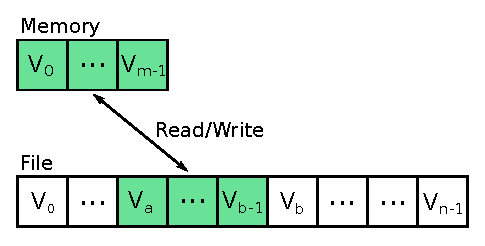
\includegraphics[scale=0.8]{pictures/HDF5Hyperslab.eps}
        }
        \hspace{0.5cm}
        \subfigure[Using hyperslab functionality to read or write dataset in parallel]{%
            \label{fig:shortColumnInCircuit}
            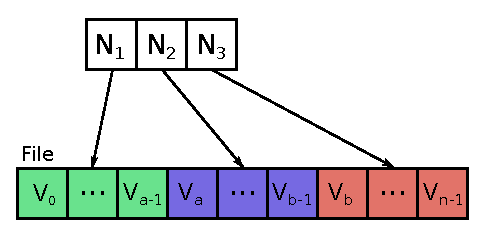
\includegraphics[scale=0.8]{pictures/HDF5Parallel.eps}
            \label{fig:hdf5hyperslabs:parallel}
       }
  
    	   \end{center}
    	\caption{%
        Using HDF5 in parallel 
     }%
   \label{fig:hdf5hyperslabs}
   \end{figure}
Parallel HDF5 is a configuration of the HDF5 library which lets you share open files across multiple parallel processes. It uses the MPI (Message Passing Interface) standard for interprocess communication. The parallel HDF5 library offers functionality to read and write from file collectively and independently.
Using hyperslab selections each process can access separate parts of a dataset \ref{fig:hdf5hyperslabs:parallel}.

\section{Task description}
In the second chapter,.. 
